
\documentclass{article}
% \usepackage{amsmath}
\usepackage[margin=0.8in]{geometry}
\usepackage{graphicx} % Required for inserting images
\usepackage{listings}
\usepackage{color}
\usepackage{verbatim} 
\usepackage{fancyvrb}
\usepackage{fvextra}



\graphicspath{ {./gtkwave/} }

\definecolor{dkgreen}{rgb}{0,0.6,0}
\definecolor{gray}{rgb}{0.5,0.5,0.5}
\definecolor{mauve}{rgb}{0.58,0,0.82}

\lstset{frame=tb,
  language=Verilog,
  aboveskip=3mm,
  belowskip=3mm,
  showstringspaces=false,
  columns=flexible,
  basicstyle={\small\ttfamily},
  numbers=none,
  numberstyle=\tiny\color{gray},
  keywordstyle=\color{blue},
  commentstyle=\color{dkgreen},
  stringstyle=\color{mauve},
  breaklines=true,
  breakatwhitespace=true,
  tabsize=3
}

\title{Digital Design Lab Report}
\author{Xiaokun Du}
\date{February 2023}

\begin{document}

% Creates a title based on the \title, \author, and \date provided
\maketitle


\section{Arithmetic logic unit (ALU)}

Write, as a SystemVerilog module with the name alu, a behavioural description of an arithmetic logic unit. \\
The data inputs, SrcA and SrcB, and the data output, ALUResult, are 8-bit vectors. The ALUControl input is a 2-bit vector. \\
The 1-bit output flag Zero = 1 if ALUResult == 0, else Zero = 0. The ALU carries out bitwise logical operations, and addition and subtraction operations, as specified in the table below.
\subsection{Module Code}
\begin{lstlisting}
module alu(input logic [7:0] SrcA,
            input logic [7:0] SrcB,
            input logic [1:0] ALUControl,
            output logic [7:0] ALUResult,
            output logic Zero);
always_comb
case (ALUControl)
2'b00 : ALUResult = SrcA & SrcB;
2'b01 : ALUResult = SrcA | SrcB;
2'b10 : ALUResult = SrcA + SrcB;
2'b11 : ALUResult = SrcA - SrcB;
default : ALUResult = 8'bx;
endcase

assign Zero = (ALUResult == 8'b0);
endmodule
\end{lstlisting}

\subsection{Testbench Code}
\begin{lstlisting}
`timescale 1ns/1ps 
`include "alu.sv"

module alu_tb;
logic [7:0] t_SrcA, t_SrcB;
logic [1:0] t_ALUControl;
logic [7:0] t_ALUResult;
logic t_Zero;

alu uut (t_SrcA, t_SrcB, t_ALUControl, t_ALUResult, t_Zero);

initial begin
    $dumpfile("alu_tb.vcd"); 
    $dumpvars(0, alu_tb);
    // Stimulus generator
    t_SrcA = 8'h05; t_SrcB = 8'h0A;
    t_ALUControl = 2'b00; #20;
    t_ALUControl = 2'b01; #20;
    t_ALUControl = 2'b10; #20;
    t_ALUControl = 2'b11; #20;
end

initial begin // Response monitor
    $monitor ("t_ALUControl = %b t_SrcA = %h t_SrcB = %h t_ALUResult = %b t_Zero = %d",t_ALUControl, t_SrcA, t_SrcB, t_ALUResult, t_Zero);
end
endmodule

\end{lstlisting}

\subsection{Simulations}
The simulation result using Icarus Verilog is as following:
\begin{Verbatim}
VCD info: dumpfile alu_tb.vcd opened for output.
t_ALUControl = 00 t_SrcA = 05 t_SrcB = 0a t_ALUResult = 00000000 t_Zero = 1
t_ALUControl = 01 t_SrcA = 05 t_SrcB = 0a t_ALUResult = 00001111 t_Zero = 0
t_ALUControl = 10 t_SrcA = 05 t_SrcB = 0a t_ALUResult = 00001111 t_Zero = 0
t_ALUControl = 11 t_SrcA = 05 t_SrcB = 0a t_ALUResult = 11111011 t_Zero = 0
\end{Verbatim}
The simulation results using GTKWave is as following:\vspace{5pt}\\
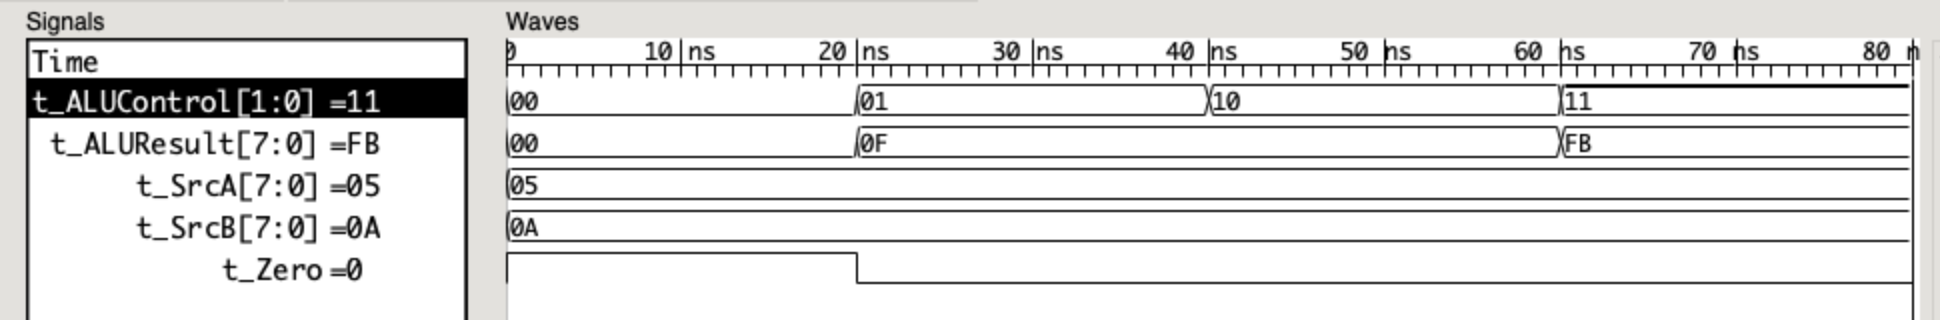
\includegraphics[width=\textwidth]{alu.png}

\newpage
\section{Register File}
The register file has sixteen 8-bit registers. The register with address 0 always contains the value 0. The other 15 registers can have values written into them through the WD3 port.\\
The contents of any two of the registers (with addresses specifiedby the 4-bit inputs RA1 and RA) are continuously output as RD1 and RD2. On the positive edge of the clock, if write\_enable is asserted, and A3 > 0, the input ALUResult is written into the register at address A3 through the WD3 port. The module includes an output port cpu\_out, which continuously outputs the contents of the register at address 15. This will form the main external output of the microprocessor.
\subsection{Module Code}
\begin{lstlisting}
module reg_file(input logic [3:0] RA1, RA2, WA, 
                input logic [7:0] ALUResult,
                input logic clk, write_enable,
                output logic [7:0] RD1, RD2, cpu_out); 
logic [7:0] rf [0:15];

assign RD1 = rf[RA1]; 
assign RD2 = rf[RA2]; 
assign cpu_out = rf[15];

// register with adress 0 always 0
initial begin
rf[4'b0] = 8'b0;
end

always_ff @(posedge clk) 
if (write_enable && WA > 0) 
rf[WA] <= ALUResult;

endmodule 
\end{lstlisting}
\subsection{Testbench Code}
\begin{lstlisting}
`timescale 1ps/1ps 
`include "reg_file.sv"

module reg_file_tb;
logic [3:0] RA1, RA2, WA;
logic clk, write_enable;
logic [7:0] ALUResult, RD1, RD2, cpu_out;
reg_file dut (RA1, RA2, WA, ALUResult, clk, write_enable, RD1, RD2, cpu_out);

initial begin // Generate clock signal with 20 ns period
    clk = 0;
    forever #10 clk = ~clk;
end

initial begin // Apply stimulus 
    $dumpfile("reg_file_tb.vcd");
    $dumpvars(0, reg_file_tb);
    RA1 = 1; RA2 = 2; WA = 0; ALUResult = 5; write_enable = 0; 
    #15 write_enable = 1;
    #20 WA = 1; ALUResult = 7;
    #20 WA = 5; ALUResult = 13;
    #20 write_enable = 0;
    #10 RA2 = 5;
    #10;
    #10 WA = 15; write_enable = 1;
    #10 ALUResult = 15;
    #30;
    $finish; // This system tasks ends the simulation 
end

initial begin // Response monitor
    $monitor ("t = %3d, t_RA1 = %d t_RA2 = %d t_WA = %d ALUResult = %d t_clk = %d t_write_enable = %d t_RD1 = %d t_RD2 = %d t_cpu_out = %d",
            $time, RA1, RA2, WA, ALUResult, clk,  write_enable, RD1, RD2, cpu_out);
end
endmodule
\end{lstlisting}

\subsection{Simulations}
The simulation results using Icarus Verilog is as below:
\begin{Verbatim}[fontsize = \footnotesize]
t =   0, RA1 =  1 RA2 =  2 WA =  0 ALUResult =   5 clk = 0 write_enable = 0 RD1 =   x RD2 =   x cpu_out =   x
t =  10, RA1 =  1 RA2 =  2 WA =  0 ALUResult =   5 clk = 1 write_enable = 0 RD1 =   x RD2 =   x cpu_out =   x
t =  15, RA1 =  1 RA2 =  2 WA =  0 ALUResult =   5 clk = 1 write_enable = 1 RD1 =   x RD2 =   x cpu_out =   x
t =  20, RA1 =  1 RA2 =  2 WA =  0 ALUResult =   5 clk = 0 write_enable = 1 RD1 =   x RD2 =   x cpu_out =   x
t =  30, RA1 =  1 RA2 =  2 WA =  0 ALUResult =   5 clk = 1 write_enable = 1 RD1 =   x RD2 =   x cpu_out =   x
t =  35, RA1 =  1 RA2 =  2 WA =  1 ALUResult =   7 clk = 1 write_enable = 1 RD1 =   x RD2 =   x cpu_out =   x
t =  40, RA1 =  1 RA2 =  2 WA =  1 ALUResult =   7 clk = 0 write_enable = 1 RD1 =   x RD2 =   x cpu_out =   x
t =  50, RA1 =  1 RA2 =  2 WA =  1 ALUResult =   7 clk = 1 write_enable = 1 RD1 =   7 RD2 =   x cpu_out =   x
t =  55, RA1 =  1 RA2 =  2 WA =  5 ALUResult =  13 clk = 1 write_enable = 1 RD1 =   7 RD2 =   x cpu_out =   x
t =  60, RA1 =  1 RA2 =  2 WA =  5 ALUResult =  13 clk = 0 write_enable = 1 RD1 =   7 RD2 =   x cpu_out =   x
t =  70, RA1 =  1 RA2 =  2 WA =  5 ALUResult =  13 clk = 1 write_enable = 1 RD1 =   7 RD2 =   x cpu_out =   x
t =  75, RA1 =  1 RA2 =  2 WA =  5 ALUResult =  13 clk = 1 write_enable = 0 RD1 =   7 RD2 =   x cpu_out =   x
t =  80, RA1 =  1 RA2 =  2 WA =  5 ALUResult =  13 clk = 0 write_enable = 0 RD1 =   7 RD2 =   x cpu_out =   x
t =  85, RA1 =  1 RA2 =  5 WA =  5 ALUResult =  13 clk = 0 write_enable = 0 RD1 =   7 RD2 =  13 cpu_out =   x
t =  90, RA1 =  1 RA2 =  5 WA =  5 ALUResult =  13 clk = 1 write_enable = 0 RD1 =   7 RD2 =  13 cpu_out =   x
t = 100, RA1 =  1 RA2 =  5 WA =  5 ALUResult =  13 clk = 0 write_enable = 0 RD1 =   7 RD2 =  13 cpu_out =   x
t = 105, RA1 =  1 RA2 =  5 WA = 15 ALUResult =  13 clk = 0 write_enable = 1 RD1 =   7 RD2 =  13 cpu_out =   x
t = 110, RA1 =  1 RA2 =  5 WA = 15 ALUResult =  13 clk = 1 write_enable = 1 RD1 =   7 RD2 =  13 cpu_out =  13
t = 115, RA1 =  1 RA2 =  5 WA = 15 ALUResult =  15 clk = 1 write_enable = 1 RD1 =   7 RD2 =  13 cpu_out =  13
t = 120, RA1 =  1 RA2 =  5 WA = 15 ALUResult =  15 clk = 0 write_enable = 1 RD1 =   7 RD2 =  13 cpu_out =  13
t = 130, RA1 =  1 RA2 =  5 WA = 15 ALUResult =  15 clk = 1 write_enable = 1 RD1 =   7 RD2 =  13 cpu_out =  15
t = 140, RA1 =  1 RA2 =  5 WA = 15 ALUResult =  15 clk = 0 write_enable = 1 RD1 =   7 RD2 =  13 cpu_out =  15 
\end{Verbatim}
The simulation results using GTKWave is as following:\vspace{5pt}\\
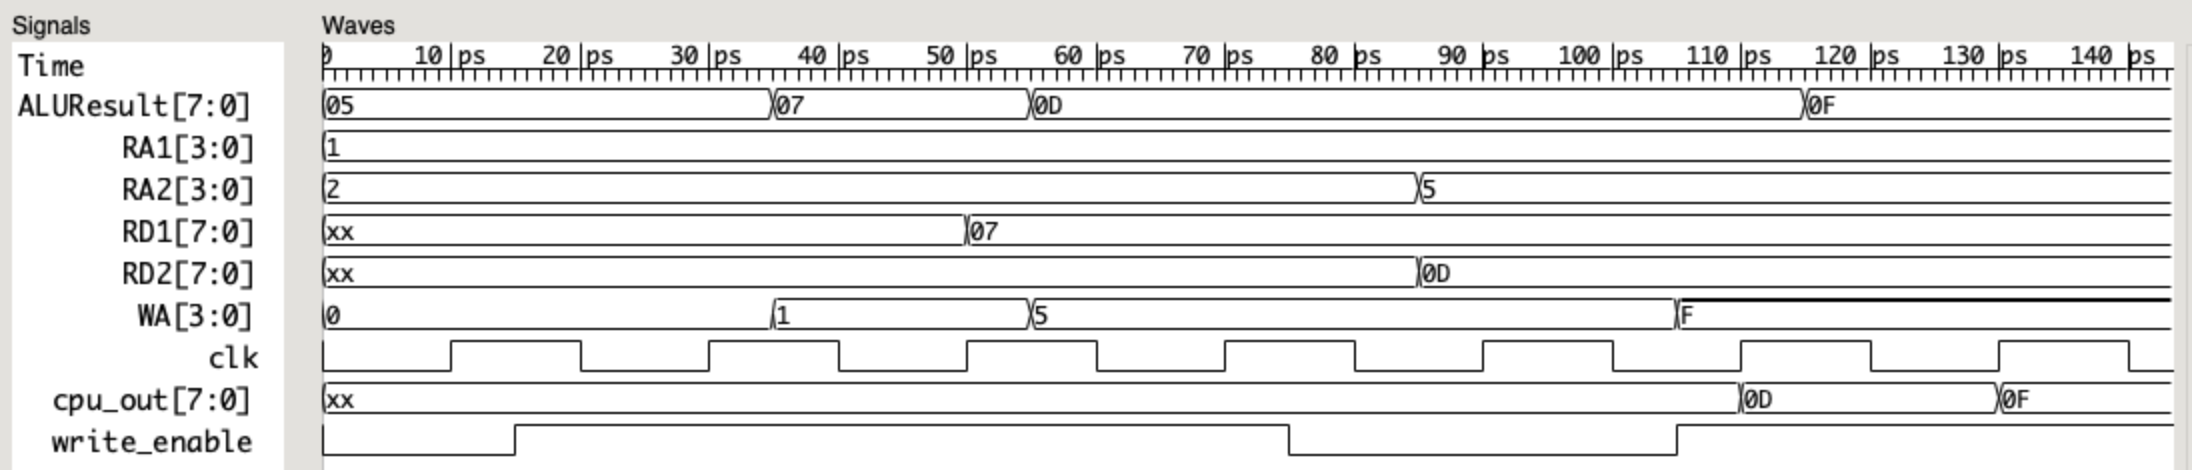
\includegraphics[width=\textwidth]{reg_file.png}

\newpage
\section{Combining the ALU and register file}
Write a SystemVerilog module with the name reg\_file\_alu, implementing the combined ALU and register file as shown above.
Include a 2-to-1 multiplexer, which selects either the RD2 output from the register file, or an external input (immediate) to be input to the ALU input port SrcB.

\subsection{Module Code}
\begin{lstlisting}
`include "reg_file.sv"
`include "alu.sv"

module reg_file_alu(input logic [3:0] RA1, RA2, WA,
                    input logic [7:0] immediate,
                    input logic [1:0] ALUControl,
                    input logic write_enable, ALUSrc, CLK,
                    output logic [7:0] ALUResult, cpu_out,
                    output logic Zero);
logic[7:0] x_srcA, x_srcB, x_RD2;

alu newalu(x_srcA, x_srcB, ALUControl, ALUResult, Zero);
reg_file newregfile(RA1, RA2, WA, ALUResult, CLK, write_enable, x_srcA, x_RD2, cpu_out);
// 2 to 1 multiplexer
assign x_srcB = (ALUSrc) ? immediate : x_RD2;

endmodule
\end{lstlisting}
\subsection{Testbench Code}
\begin{lstlisting}
`timescale 1ps/1ps 
`include "reg_file_alu.sv"

module reg_file_alu_tb;
logic [3:0] t_RA1, t_RA2, t_WA;
logic [7:0] t_immediate, t_ALUResult, t_cpu_out;
logic [1:0] t_ALUControl;
logic t_write_enable, t_ALUSrc, clk, t_Zero;

reg_file_alu dut (t_RA1, t_RA2, t_WA, t_immediate, t_ALUControl, t_write_enable, t_ALUSrc, clk, 
                t_ALUResult, t_cpu_out, t_Zero);

initial begin
    clk = 0;
    forever #10 clk = ~clk;
end

initial begin // Apply stimulus 
    $dumpfile("reg_file_alu_tb.vcd");
    $dumpvars(0, reg_file_alu_tb);
    t_RA1 = 4'h0; t_RA2 = 4'h2; t_WA = 4'h0; t_immediate = 8'h0A; 
    t_ALUSrc = 1; t_ALUControl = 2'b10; t_write_enable = 1;
    #10 t_RA2 = 4'h1; t_WA = 4'h1;
    #10 t_immediate = 8'h07;
    #20 t_RA1 = 4'h1; t_WA = 4'h1;
    #40 t_ALUControl = 2'b11; t_WA = 4'hF;
    #20 t_immediate = 8'b10111111;
    #20 t_immediate = 8'h0; t_ALUControl = 2'b00;
    #10

$finish; // This system tasks ends the simulation 
end

initial begin // Response monitor
    $monitor ("t = %3d, RA1 = %d RA2 = %d WA = %d Immediate = %d clk = %d write_enable = %d alusRC = %d alucontrol = %d aluresult = %d cpu_out = %d zero = %d",
            $time, t_RA1, t_RA2, t_WA, t_immediate, clk,  t_write_enable, t_ALUSrc, t_ALUControl, t_ALUResult, t_cpu_out, t_Zero);
end
endmodule
\end{lstlisting}

\subsection{Simulations}
The simulation result using Icarus Verilog is as following:
\begin{Verbatim}[fontsize = \scriptsize]
VCD info: dumpfile reg_file_alu_tb.vcd opened for output.
t =   0, RA1 =  0 RA2 =  2 WA =  0 Immediate =  10 clk = 0 write_enable = 1 alusRC = 1 alucontrol = 2 aluresult =  10 cpu_out =   x zero = 0
t =  10, RA1 =  0 RA2 =  1 WA =  1 Immediate =  10 clk = 1 write_enable = 1 alusRC = 1 alucontrol = 2 aluresult =  10 cpu_out =   x zero = 0
t =  20, RA1 =  0 RA2 =  1 WA =  1 Immediate =   7 clk = 0 write_enable = 1 alusRC = 1 alucontrol = 2 aluresult =   7 cpu_out =   x zero = 0
t =  30, RA1 =  0 RA2 =  1 WA =  1 Immediate =   7 clk = 1 write_enable = 1 alusRC = 1 alucontrol = 2 aluresult =   7 cpu_out =   x zero = 0
t =  40, RA1 =  1 RA2 =  1 WA =  1 Immediate =   7 clk = 0 write_enable = 1 alusRC = 1 alucontrol = 2 aluresult =  14 cpu_out =   x zero = 0
t =  50, RA1 =  1 RA2 =  1 WA =  1 Immediate =   7 clk = 1 write_enable = 1 alusRC = 1 alucontrol = 2 aluresult =  21 cpu_out =   x zero = 0
t =  60, RA1 =  1 RA2 =  1 WA =  1 Immediate =   7 clk = 0 write_enable = 1 alusRC = 1 alucontrol = 2 aluresult =  21 cpu_out =   x zero = 0
t =  70, RA1 =  1 RA2 =  1 WA =  1 Immediate =   7 clk = 1 write_enable = 1 alusRC = 1 alucontrol = 2 aluresult =  28 cpu_out =   x zero = 0
t =  80, RA1 =  1 RA2 =  1 WA = 15 Immediate =   7 clk = 0 write_enable = 1 alusRC = 1 alucontrol = 3 aluresult =  14 cpu_out =   x zero = 0
t =  90, RA1 =  1 RA2 =  1 WA = 15 Immediate =   7 clk = 1 write_enable = 1 alusRC = 1 alucontrol = 3 aluresult =  14 cpu_out =  14 zero = 0
t = 100, RA1 =  1 RA2 =  1 WA = 15 Immediate = 191 clk = 0 write_enable = 1 alusRC = 1 alucontrol = 3 aluresult =  86 cpu_out =  14 zero = 0
t = 110, RA1 =  1 RA2 =  1 WA = 15 Immediate = 191 clk = 1 write_enable = 1 alusRC = 1 alucontrol = 3 aluresult =  86 cpu_out =  86 zero = 0
t = 120, RA1 =  1 RA2 =  1 WA = 15 Immediate =   0 clk = 0 write_enable = 1 alusRC = 1 alucontrol = 0 aluresult =   0 cpu_out =  86 zero = 1
t = 130, RA1 =  1 RA2 =  1 WA = 15 Immediate =   0 clk = 1 write_enable = 1 alusRC = 1 alucontrol = 0 aluresult =   0 cpu_out =   0 zero = 1
\end{Verbatim}
The simulation results using GTKWave is as following:\vspace{5pt}\\
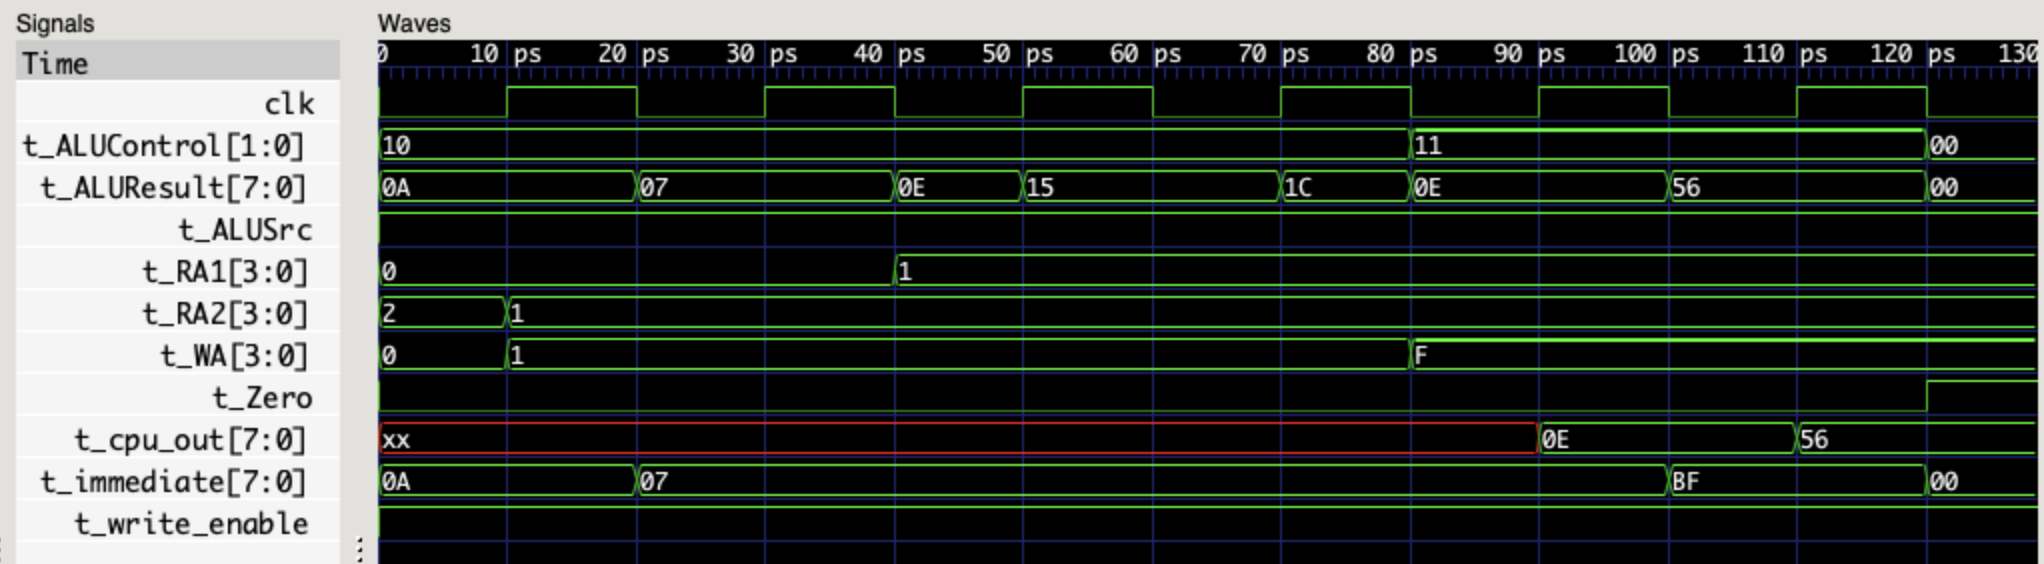
\includegraphics[width=\textwidth]{reg_file_alu.png}

\newpage
\section{Instruction memory}

\subsection{Module Code}
\begin{lstlisting}
module instruction_memory(input logic[7:0] PC,
                            output logic[23:0] Instr);
logic [23:0] data_ROM [0:256];
initial
$readmemh("program.txt", data_ROM); 
assign Instr = data_ROM[PC]; 
endmodule
\end{lstlisting}

\subsection{Text File}
This is the content of the text file named ``program.txt'':
\begin{Verbatim}
610001
620020
6F0000
701207
211100
6FF001
700003
700007
\end{Verbatim}

\subsection{Testbench Code}
\begin{lstlisting}
`timescale 1ns/1ps 
`include "instruction_memory.sv"

module instruction_memory_tb;
logic [7:0] t_PC;
logic [23:0] t_Instr;

instruction_memory dut (t_PC, t_Instr);

initial begin
    $dumpfile("instruction_memory_tb.vcd"); 
    $dumpvars(0, instruction_memory_tb);
    // Stimulus generator
    t_PC = 8'h00; 
    #10 t_PC = 8'h01;
    #10 t_PC = 8'h02;
    #10 t_PC = 8'h03;
    #10 t_PC = 8'h04;
    #10 t_PC = 8'h05;
    #10 t_PC = 8'h06;
    #10 t_PC = 8'h07;
    
end

initial begin // Response monitor
    $monitor ("t_PC = %h t_Instr = %h", t_PC, t_Instr);
end

endmodule
\end{lstlisting}

\subsection{Simulations}
The simulation result using Icarus Verilog is as following:
\begin{Verbatim}
    t_PC = 00 t_Instr = 610001
    t_PC = 01 t_Instr = 620020
    t_PC = 02 t_Instr = 6f0000
    t_PC = 03 t_Instr = 701207
    t_PC = 04 t_Instr = 211100
    t_PC = 05 t_Instr = 6ff001
    t_PC = 06 t_Instr = 700003
    t_PC = 07 t_Instr = 700007
\end{Verbatim}

\newpage
\section{Program Counter}
Implement the 8-bit program counter shown above, as a SystemVerilog module with the name pc. The register should be updated on the positive edges of the clock, and have an active high reset. The 2-to-1 multiplexer selects the next value of PC as either PC+1 (the next instruction in the program will be fetched) or the input immediate (the program branches to an instruction elsewhere).

\subsection{Module Code}
\begin{lstlisting}
module pc (input logic[7:0] immediate, 
            input logic PCSrc, CLK, reset,
            output logic[7:0] PC);
always_ff @ (posedge CLK) begin
    if (reset) PC <= 8'b0; 
    else if (PCSrc) PC <= immediate;
    else PC <= PC + 1; 
end
endmodule
\end{lstlisting}

\subsection{Testbench Code}
\begin{lstlisting}
`timescale 1ns/1ps
`include "pc.sv"

module pc_tb;
logic [7:0] t_PC, t_immediate;
logic t_PCSrc, clk, t_reset;

pc pc(t_immediate, t_PCSrc, clk, t_reset, t_PC);

initial begin
    clk = 0;
    forever #10 clk = ~clk;
end

initial begin
    $dumpfile("pc_tb.vcd"); 
    $dumpvars(0, pc_tb);
    // Stimulus generator
    t_reset = 1; t_PCSrc = 0; t_immediate = 8'b01;
    #10 t_reset = 0; t_PCSrc = 1;
    #20 t_immediate = 8'b111;
    #20 t_PCSrc = 0;
    #50 t_reset = 1;
end

initial begin // Response monitor
    $monitor ("t = %3d clk = %d, t_immediate = %b t_PCSrc = %b t_reset = %d t_PC = %d", $time, clk, t_immediate, t_PCSrc, t_reset, t_PC);
    #120;
    $finish; 
end

endmodule
\end{lstlisting}

\subsection{Simulations}
The simulation result using Icarus Verilog is as following:
\begin{Verbatim}
t =   0 clk = 0, t_immediate = 00000001 t_PCSrc = 0 t_reset = 1 t_PC =   x
t =  10 clk = 1, t_immediate = 00000001 t_PCSrc = 1 t_reset = 0 t_PC =   1
t =  20 clk = 0, t_immediate = 00000001 t_PCSrc = 1 t_reset = 0 t_PC =   1
t =  30 clk = 1, t_immediate = 00000111 t_PCSrc = 1 t_reset = 0 t_PC =   7
t =  40 clk = 0, t_immediate = 00000111 t_PCSrc = 1 t_reset = 0 t_PC =   7
t =  50 clk = 1, t_immediate = 00000111 t_PCSrc = 0 t_reset = 0 t_PC =   8
t =  60 clk = 0, t_immediate = 00000111 t_PCSrc = 0 t_reset = 0 t_PC =   8
t =  70 clk = 1, t_immediate = 00000111 t_PCSrc = 0 t_reset = 0 t_PC =   9
t =  80 clk = 0, t_immediate = 00000111 t_PCSrc = 0 t_reset = 0 t_PC =   9
t =  90 clk = 1, t_immediate = 00000111 t_PCSrc = 0 t_reset = 0 t_PC =  10
t = 100 clk = 0, t_immediate = 00000111 t_PCSrc = 0 t_reset = 1 t_PC =  10
t = 110 clk = 1, t_immediate = 00000111 t_PCSrc = 0 t_reset = 1 t_PC =   0
t = 120 clk = 0, t_immediate = 00000111 t_PCSrc = 0 t_reset = 1 t_PC =   0
\end{Verbatim}
The simulation results using GTKWave is as following:\vspace{5pt}\\
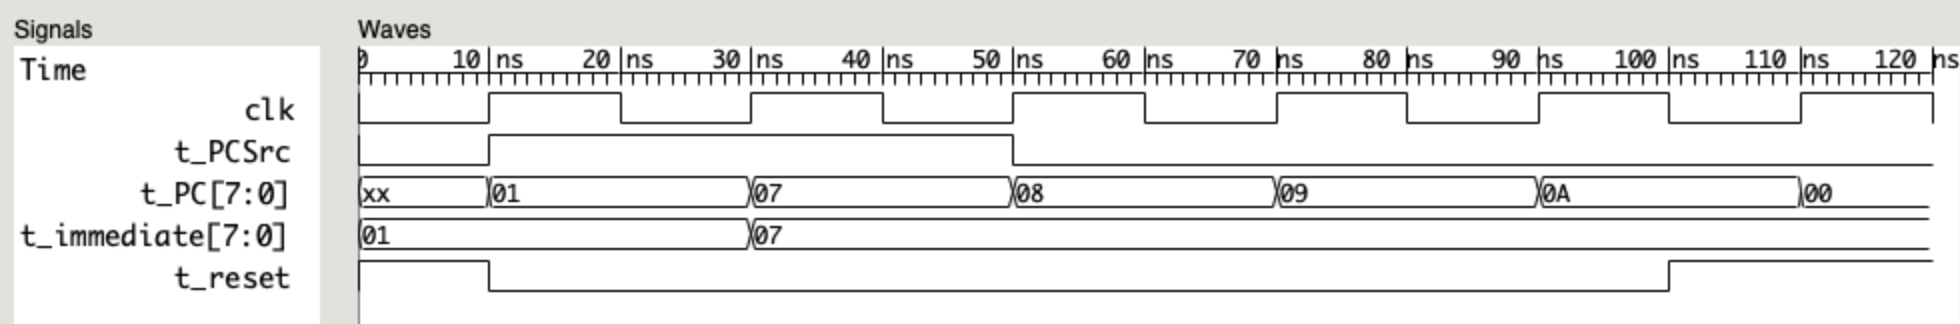
\includegraphics[width=\textwidth]{pc.png}

\newpage
\section{Combining the ROM with program counter}
\subsection{Module Code}




\end{document}
